%! TeX root = ../main.tex

\chapter{Code Tutorial}%
\label{app:code-tutorial}

Here, we show the tutorial of the package \texttt{RAS\_DMFT.jl} version 0.10.0.
An up-to-date guide is available in the package documentation.


\section{Non-interacting Bethe lattice in infinite dimensions}

The non-interacting density is the Wigner semicircle distribution
\begin{equation}
    \rho(\omega) = \frac{2}{\muppi D^2}\sqrt{D^2 - \omega^2}
\end{equation}
from which we can define a non-interacting Green's function $G(\omega)$ with the relation
\begin{equation}
    \rho(\omega) = -\frac{1}{\muppi}\Im G(\omega).
\end{equation}
Let us plot it:
\begin{minted}[
        autogobble,
    ]{julia}
        D = 1.0 # half-bandwith
        W = range(-2 * D, 2 * D; length = 1_000) # frequency grid
        g = greens_function_bethe_analytic(W, D)

        f = Figure();
        ax = Axis(f[1, 1]; xlabel = L"ω/D", ylabel = L"DG")
        lines!(ax, W, real(g); label = L"\mathrm{Re}~G_0")
        lines!(ax, W, imag(g); label = L"\mathrm{Im}~G_0")
        axislegend(ax; position = :lt)
        xlims!(ax, first(W), last(W))
\end{minted}
\begin{center}
    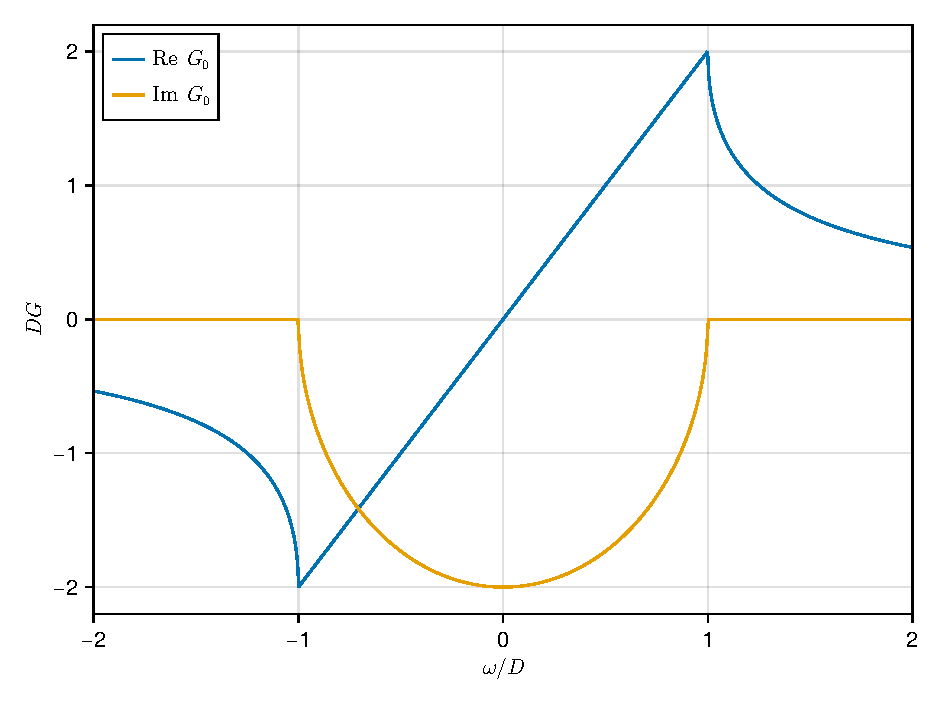
\includegraphics[width=0.7\textwidth]{graphics/tutorial1.pdf}
\end{center}
For calculations, we need to discretize this to $N$ points:
\begin{minted}[
        autogobble,
    ]{julia}
        N = 51 # number of points
        grid = range(-D, D; length = N) # linear grid (others are possible)
        G0 = greens_function_bethe_grid(grid)
\end{minted}
This returns a \texttt{PoleSum} instance which only stores locations $\epsilon_i$
and weights $w_i$.
\begin{minted}[
        autogobble,
    ]{julia}
        f = Figure();
        ax = Axis(f[1, 1]; xlabel = "locations", ylabel = "weights")
        plot!(ax, locations(G0), weights(G0))
\end{minted}
\begin{center}
    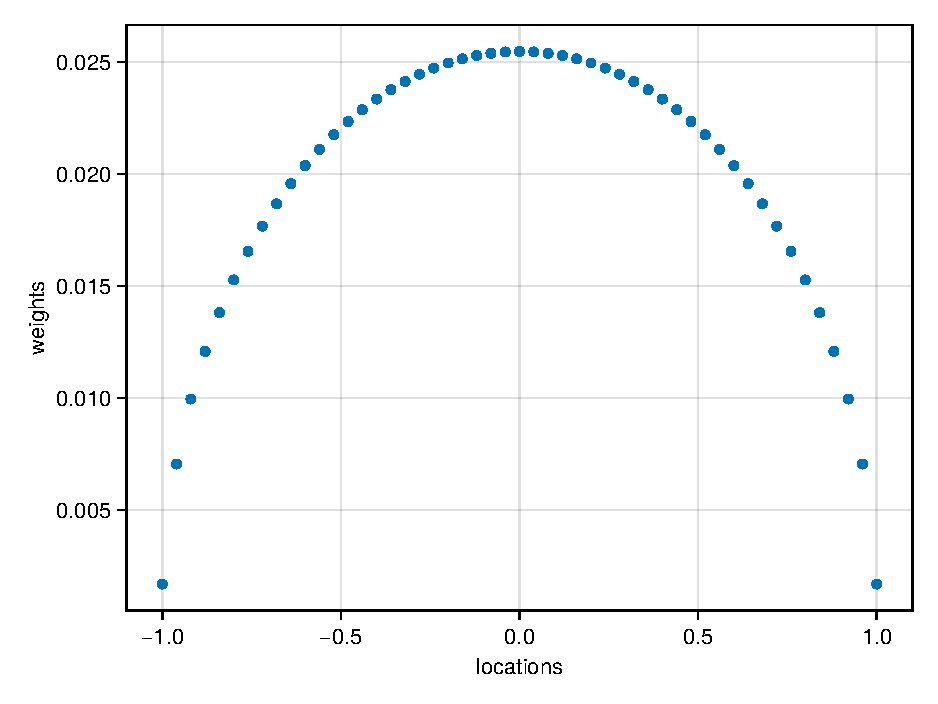
\includegraphics[width=0.7\textwidth]{graphics/tutorial2.pdf}
\end{center}
We can see that this looks like a discrete version of our semicircle.
Our spectrum is now
\begin{equation}
    A(\omega) = \sum_i w_i \delta(\omega - \epsilon_i).
\end{equation}
If we introduce some broadening, this should look like the continuous one.
Lorentzian broadening is characterized by $δ$
\begin{equation}
    A(\omega) = \sum_i w_i \frac{1}{\muppi}\frac{\delta}{(\omega -\epsilon_i)^2 + \delta^2},
\end{equation}
Gaussian one by $\sigma$
\begin{equation}
    A(\omega)
    =
    \sum_i
    w_i\frac{1}{\sqrt{2\muppi\sigma^2}}
    \exp\left(-\frac{(\omega - \epsilon_i)^2}{2\sigma^2}\right).
\end{equation}
\begin{minted}[
        autogobble,
    ]{julia}
        δ = σ = 0.04
        f = Figure();
        ax = Axis(f[1, 1]; xlabel = L"ω/D", ylabel = L"πDA(ω)")
        lines!(ax, W, -imag(g); label = "exact", color = :gray, linewidth = 4)
        lines!(ax, W, -imag(evaluate_lorentzian(G0, W, δ)); label = "Lorentzian")
        lines!(ax, W, -imag(evaluate_gaussian(G0, W, σ)); label = "Gaussian")
        axislegend(ax; position = :lt)
        xlims!(ax, first(W), last(W))
\end{minted}
\begin{center}
    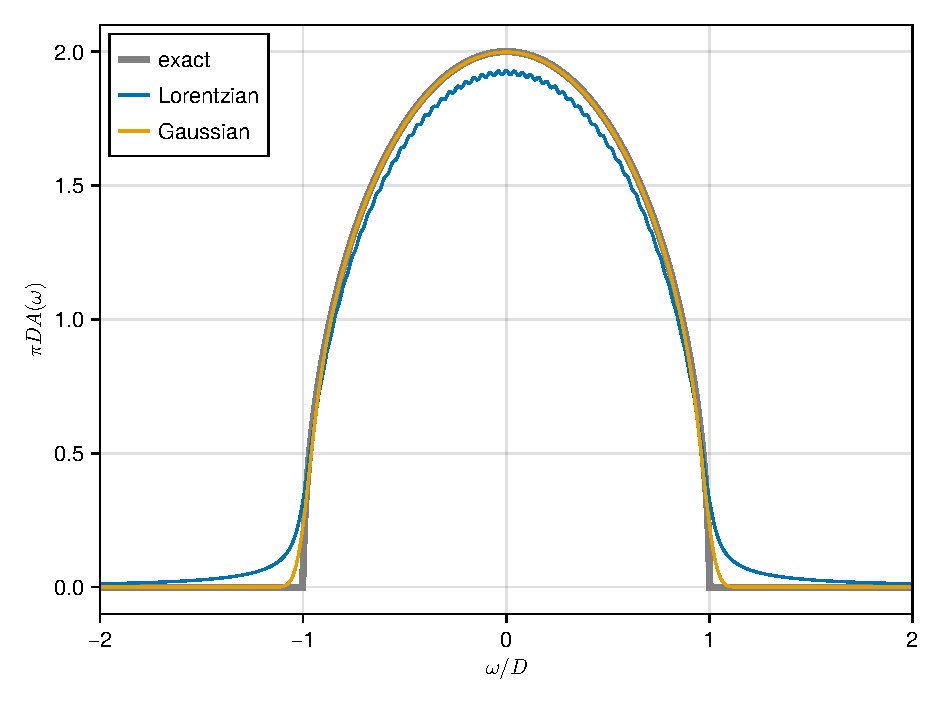
\includegraphics[width=0.7\textwidth]{graphics/tutorial3.pdf}
\end{center}

\pagebreak % looks nicer
\section{DMFT step}

For all following calculations we set our unit of energy to $D=1$.

\subsection{Impurity}
Values for the half-filled impurity.
A value of $U/D=2.0$ will generate a strongly correlated metal.
\begin{minted}[
        autogobble,
    ]{julia}
        U = 2.0 # Coulomb interaction
        μ = U / 2 # chemical potential
        ϵ_imp = -μ # energy level for half-filling
        # Restrictions for our active space.
        L = 1 # number of chain sites to be treated exactly
        p = 2 # order of excitations for remaining chains
\end{minted}
Operators for exact part.
This is necessary to introduce the interacting part and Hartree term.
One can also introduce other operators, e.g., $S_z$, $S^2$
and measure their expectation values.
\begin{minted}[
        autogobble,
    ]{julia}
        fs = FockSpace(Orbitals(2 + 2 * L), FermionicSpin(1 // 2))
        c = annihilators(fs)
        n = occupations(fs)
        H_int = U * n[1, 1 // 2] * n[1, -1 // 2] # interacting Hamiltonian
        d_dag = c[1, -1 // 2]' # d_↓^†
        q_dag = H_int * d_dag - d_dag * H_int  # auxiliary operator q_↓^† = [H_int, d^†]
        # measure these on ground state
        O_Σ_H = q_dag' * d_dag + d_dag * q_dag' # Operator for Hartree term
        d_occ = n[1, 1 // 2] * n[1, -1 // 2] # double occupation
\end{minted}

\subsection{Hybridization function}

On the Bethe lattice,
the hybridization function $Δ$ is nothing more than a rescaled Green's function
\begin{equation}
    \Delta(\omega) = \frac{D^2}{4} G(\omega).
\end{equation}
We can create one using
\begin{minted}[
        autogobble,
    ]{julia}
        n_bath = 51 # number of bath sites
        grid = range(-4 * D, 4 * D; length = N) # linear grid
        Δ0 = hybridization_function_bethe_grid(grid)
        remove_zero_weight!(Δ0)
\end{minted}
Here, we set our grid to $[-4D, 4D]$.
This will initially create poles with zero weight.
Due to the Coulomb interaction $U$, spectral weight will move to higher frequencies,
such that poles with initially no weight will obtain a finite value
in successive calculations.

\subsection{Ground state}%
\label{app:tutorial_ground-state}

We can then calculate the ground state
up to a user-given variance of the Hamiltonian $\var(H)$.
\begin{minted}[
        autogobble,
    ]{julia}
        var = 1.0e-10
        H, E0, ψ0 = init_system(Δ0, H_int, ϵ_imp, L, L, p, var);
        # Given our ground state,
        # we can calculate expectation values with `LinearAlgebra.dot`.
        dot(ψ0, d_occ, ψ0) # expectation value
        Σ_H = dot(ψ0, O_Σ_H, ψ0) # Hartree term, should be U/2 = 1.0
\end{minted}

\subsection{Block correlator}

Shift to create diagonal matrices later.
\begin{minted}[
        autogobble,
    ]{julia}
        q_dag_tilde = q_dag - Σ_H * d_dag
        O_plus = [q_dag_tilde, d_dag] # for C+
        O_minus = map(adjoint, O_plus); # for C-
\end{minted}
As we have two operators as input, we will create $2\times2$ block correlators.
If we use $n$ Krylov steps, each will have $2n$ poles.
\begin{minted}[
        autogobble,
    ]{julia}
        n_kryl = 50
        C_plus = correlator_plus(H, ψ0, O_plus, n_kryl)
        C_minus = correlator_minus(H, ψ0, O_minus, n_kryl)
        C = transpose(C_minus) + C_plus
\end{minted}
We can plot the spectrum.
The Green's function is the $[2,2]$ component.
\begin{minted}[
        autogobble,
    ]{julia}
        G = PolesSum(C, 2, 2)
        f = Figure();
        ax = Axis(f[1, 1]; xlabel = L"ω/D", ylabel = L"πDA(ω)")
        lines!(ax, W, -imag(evaluate_gaussian(G, W, σ)))
        xlims!(ax, first(W), last(W))
\end{minted}
\begin{center}
    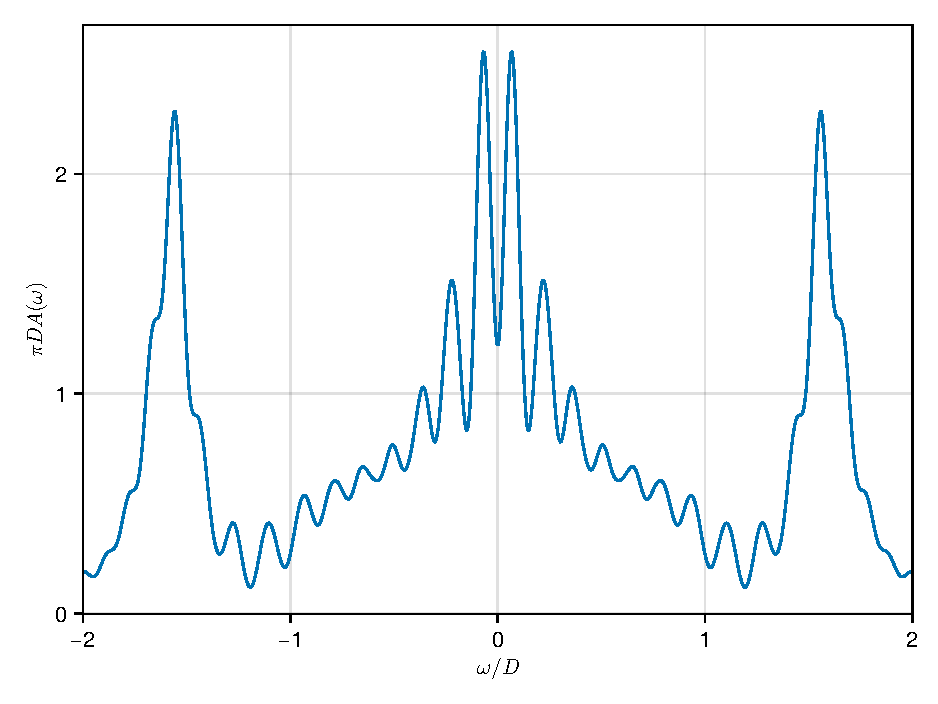
\includegraphics[width=0.7\textwidth]{graphics/tutorial4.pdf}
\end{center}

\subsection{Self-energy}

Here, we use the improved symmetric estimator~\cite{Kugler2022} $\Sigma^\mIFG$.
\begin{minted}[
        autogobble,
    ]{julia}
        Σ = self_energy_IFG(C)
        sigma = evaluate_gaussian(Σ, W, σ)
        f = Figure();
        ax = Axis(f[1, 1]; xlabel = L"ω/D", ylabel = L"Σ(ω)/D")
        lines!(ax, W, real(sigma); label = L"\mathrm{Re}~Σ")
        lines!(ax, W, imag(sigma); label = L"\mathrm{Im}~Σ")
        axislegend(ax; position = :lt)
        xlims!(ax, first(W), last(W))
\end{minted}
\begin{center}
    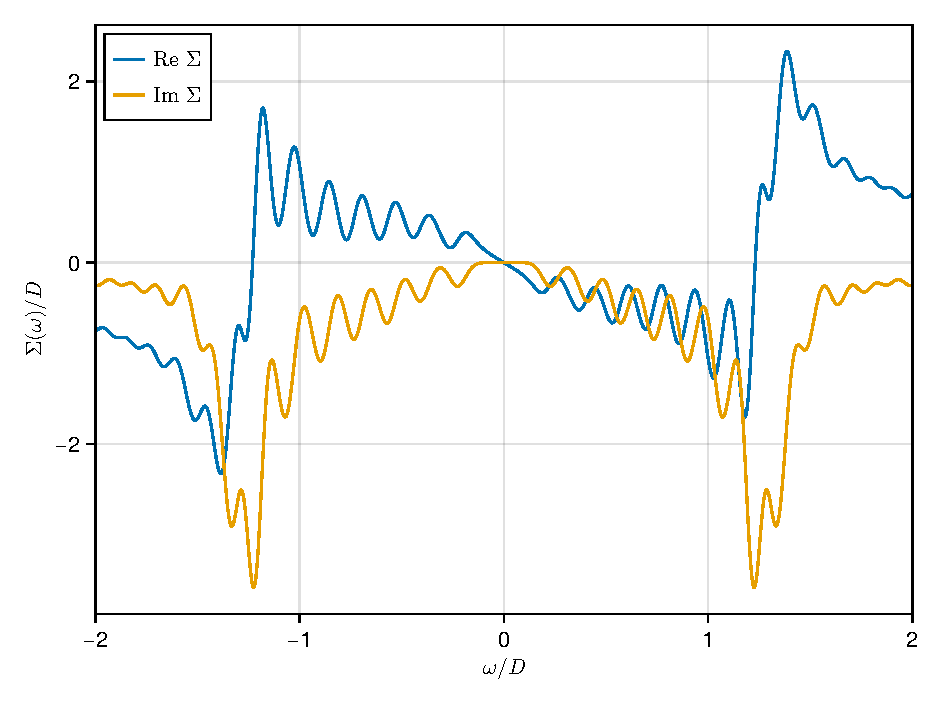
\includegraphics[width=0.7\textwidth]{graphics/tutorial5.pdf}
\end{center}

We can calculate the quasiparticle weight
\begin{align}
    Z
     & =
    \left(1 - \left.\frac{∂\mathrm{Re}~Σ}{∂ω}\right|_{ω=0}\right)^{-1} \\
     & =
    \left(1 + \sum_i \frac{w_i}{ϵ_i^2}\right)^{-1}
\end{align}
directly on the real axis without the use of a difference quotient.
Due to poles at $\epsilon_i≈0$ this will diverge,
and poles with small weight need to be ignored.
This is controlled by the second parameter.
\begin{minted}[
        autogobble,
    ]{julia}
        quasiparticle_weight(Σ, sqrt(eps()))
\end{minted}

\subsection{Update hybridization}
At the end of each DMFT step, we have to update the hybridization function
using the new self-energy.
\begin{minted}[
        autogobble,
    ]{julia}
        Δ = update_hybridization_function(Δ0, μ, Σ_H, Σ)
\end{minted}
As this function has too many poles to be computationally feasible,
we put them onto our initial grid
\begin{minted}[
        autogobble,
    ]{julia}
        Δ_grid = to_grid(Δ, grid)
\end{minted}
We can then put this as our next input and continue at \zcref{app:tutorial_ground-state}.
